%% LyX 2.3.3 created this file.  For more info, see http://www.lyx.org/.
%% Do not edit unless you really know what you are doing.
\documentclass[a4paper,english]{article}
\usepackage[T1]{fontenc}
\usepackage[latin9]{inputenc}
\usepackage{array}
\usepackage{float}
\usepackage{calc}
\usepackage{amsmath}
\usepackage{amsthm}
\usepackage{amssymb}
\usepackage{stackrel}
\usepackage{graphicx}
\usepackage{wasysym}
\PassOptionsToPackage{normalem}{ulem}
\usepackage{ulem}

\makeatletter

%%%%%%%%%%%%%%%%%%%%%%%%%%%%%% LyX specific LaTeX commands.
\pdfpageheight\paperheight
\pdfpagewidth\paperwidth

%% Because html converters don't know tabularnewline
\providecommand{\tabularnewline}{\\}
\floatstyle{ruled}
\newfloat{algorithm}{tbp}{loa}
\providecommand{\algorithmname}{Algorithm}
\floatname{algorithm}{\protect\algorithmname}

%%%%%%%%%%%%%%%%%%%%%%%%%%%%%% Textclass specific LaTeX commands.
\theoremstyle{definition}
    \ifx\thechapter\undefined
      \newtheorem{defn}{\protect\definitionname}
    \else
      \newtheorem{defn}{\protect\definitionname}[chapter]
    \fi
\theoremstyle{plain}
    \ifx\thechapter\undefined
	    \newtheorem{thm}{\protect\theoremname}
	  \else
      \newtheorem{thm}{\protect\theoremname}[chapter]
    \fi
\theoremstyle{remark}
    \ifx\thechapter\undefined
      \newtheorem{rem}{\protect\remarkname}
    \else
      \newtheorem{rem}{\protect\remarkname}[chapter]
    \fi
\theoremstyle{plain}
    \ifx\thechapter\undefined
  \newtheorem{cor}{\protect\corollaryname}
\else
      \newtheorem{cor}{\protect\corollaryname}[chapter]
    \fi
\theoremstyle{definition}
    \ifx\thechapter\undefined
      \newtheorem{example}{\protect\examplename}
    \else
      \newtheorem{example}{\protect\examplename}[chapter]
    \fi
\theoremstyle{plain}
    \ifx\thechapter\undefined
      \newtheorem{lem}{\protect\lemmaname}
    \else
      \newtheorem{lem}{\protect\lemmaname}[chapter]
    \fi
\theoremstyle{plain}
    \ifx\thechapter\undefined
      \newtheorem{conjecture}{\protect\conjecturename}
    \else
      \newtheorem{conjecture}{\protect\conjecturename}[chapter]
    \fi

%%%%%%%%%%%%%%%%%%%%%%%%%%%%%% User specified LaTeX commands.
\usepackage{placeins}
\usepackage{graphicx}

\theoremstyle{construction}
    \ifx\thechapter\undefined
      \newtheorem{constr}{\protect\constructionname}
    \else
      \newtheorem{constr}{\protect\constructionname}[chapter]
    \fi
\providecommand{\constructionname}{Construction}

\makeatother

\usepackage{babel}
\providecommand{\conjecturename}{Conjecture}
\providecommand{\corollaryname}{Corollary}
\providecommand{\definitionname}{Definition}
\providecommand{\examplename}{Example}
\providecommand{\lemmaname}{Lemma}
\providecommand{\remarkname}{Remark}
\providecommand{\theoremname}{Theorem}

\begin{document}

\part{Preliminaries}

\section{Definition}
\begin{defn}[Vector Space]
 A vector space of dimension $n$ over a finite field with $q$ elements
is denoted by $\ensuremath{\mathbb{F}}_{q}^{n}$.
\end{defn}
%
\begin{defn}[Gaussian coefficient]
 Gaussian coefficient (also known as $q$-binomial), which counts
the number of subspaces of dimension $k$ in a vector space $\ensuremath{\mathbb{F}}_{q}^{n}$:

\[
\left[\begin{array}{c}
n\\
k
\end{array}\right]_{q}=\stackrel[i=0]{k-1}{\prod}\frac{q^{n}-q^{i}}{q^{k}-q^{i}}
\]
\end{defn}
%
\begin{defn}[Grassmannian Code]
 A Grassmannian code is a set of all subspaces of dimension $k\leq n$
in $\ensuremath{\mathbb{F}}_{q}^{n}$, and is denoted by $\mathcal{G}_{q}\left(n,k\right)$.
Due to being the set of all subspaces that have the same dimension
$k$, it is also called a \textit{constant dimension code}. The cardinality
of $\mathcal{G}_{q}\left(n,k\right)$ is the Gaussian coefficient
(also known as $q$-binomial), which counts the number of subspaces
of dimension $k$ in a vector space $\ensuremath{\mathbb{F}}_{q}^{n}$:

\[
\left|\mathcal{G}_{q}\left(n,k\right)\right|=\left[\begin{array}{c}
n\\
k
\end{array}\right]_{q}=\stackrel[i=0]{k-1}{\prod}\frac{q^{n}-q^{i}}{q^{k}-q^{i}},
\]

where $q^{\left(n-k\right)k}\leq\left[\begin{array}{c}
n\\
k
\end{array}\right]_{q}\leq4q^{\left(n-k\right)k}$.
\end{defn}
%
\begin{defn}[Projective Space]
 The \textit{projective space of order} $n$ is a set of all subspaces
of $\ensuremath{\mathbb{F}}_{q}^{n}$, and is denoted by $\mathcal{P}_{q}\left(n\right)$,
i.e. a union of all dimension $k=0,\ldots n$ subspaces in $\ensuremath{\mathbb{F}}_{q}^{n}$
or $\mathcal{P}_{q}\left(n\right)=\bigcup_{k=0}^{n}\mathcal{G}_{q}\left(n,k\right)$.
\end{defn}
%
\begin{defn}[Covering Grassmannian code]
 An $\alpha-\left(n,k,\delta\right)_{q}^{c}$ covering Grassmannian
code (code in short) $\mathcal{C}$ is a subset of $\mathcal{G}_{q}\left(n,k\right)$
such that each subset of $\alpha$ codewords of $\mathcal{C}$ span
a subspace whose dimension is at least $\delta+k$ in $\ensuremath{\mathbb{F}}_{q}^{n}$.
\end{defn}
%
\begin{defn}[Multiple Grassmannian code]
 A $t-\left(n,k,\lambda\right)_{q}^{m}$ multiple Grassmannian code
(code in short) $\mathcal{C}$ is a subset of $\mathcal{G}_{q}\left(n,k\right)$
such that each $t$-subspace of $\ensuremath{\mathbb{F}}_{q}^{n}$
is contained in at most $\lambda$ codewords of $\mathcal{C}$. Following
to \cite{Zhang:2019}, $m$ refers to multiplicity.
\end{defn}
%
\begin{defn}
$\mathcal{A}_{q}\left(n,k,t;\lambda\right)$ denotes the maximum size
of a $t-\left(n,k,\lambda\right)_{q}^{m}$ code, where there are no
repeated codewords.
\end{defn}
%
\begin{defn}[Subspace packing]
 A subspace packing $t-\left(n,k,\lambda\right)_{q}^{m}$ is a set
$\mathcal{S}$ of $k$-subspaces or $k$-dimensional subspaces (called
\textit{blocks}), such that each $t$-subspace of $\ensuremath{\mathbb{F}}_{q}^{n}$
is contained in at most $\lambda$ codewords of $\mathcal{C}$.
\end{defn}

\section{Theorem}
\begin{thm}
If $n,k,t,$ and $\lambda$ are positive integers such that $1\leq t<k<n$
and $1\leq\lambda\leq\left[\begin{array}{c}
n-t\\
k-t
\end{array}\right]_{q}$, then

\[
\mathcal{A}_{q}\left(n,k,t;\lambda\right)\leq\left\lfloor \lambda\frac{\left[\begin{array}{c}
n\\
t
\end{array}\right]_{q}}{\left[\begin{array}{c}
k\\
t
\end{array}\right]_{q}}\right\rfloor 
\]
\end{thm}
%
\begin{thm}
If $n,k,t,$ and $\lambda$ are positive integers such that $1\leq t<k<n$
and $1\leq\lambda\leq\left[\begin{array}{c}
n-t\\
k-t
\end{array}\right]_{q}$, then

\[
\mathcal{A}_{q}\left(n,k,t;\lambda\right)\leq\left\lfloor \frac{q^{n}-1}{q^{k}-1}\mathcal{A}_{q}\left(n-1,k-1,t-1;\lambda\right)\right\rfloor 
\]
\end{thm}

\part{Generalized Combination Network $(\epsilon,l)-\mathcal{N}_{h,r,s}$}

\section{Description \label{sec:Description_GCN}}

A generalized combination network $(\epsilon,l)-\mathcal{N}_{h,r,s}$
consists of 3 components from top to bottom: ``Source'' in the first
layer, ``Node'' in the middle layer, and ``Receiver'' in the third
layer. The network has a source with $h$ messages, $r$ nodes, and
$\left(\begin{array}{c}
r\\
\alpha
\end{array}\right)$ receivers, which form a single source multicast network modeled as
a finite directed acyclic multigraph. The source connects to each
node by $l$ parallel links and each node also connects to a receiver
by $l$ parallel links, which are respectively called a node's incoming
and outgoing edges. Each receiver is connected by $s$ links in total,
specifically $\alpha l$ links from $\alpha$ nodes and $\epsilon$
direct links from the source, i.e. $s=\alpha l+\epsilon$. The combination
network in \cite{Riis:2006} is the $(0,1)-\mathcal{N}_{h,r,s}$ network
and the $(1,1)-\mathcal{N}_{h,r,s}$ network is called One-Direct
Link Combination Network. Theorem 1 shows our interest of relations
between the parameters $h,\alpha,\epsilon$ and $l$.
\begin{thm}
\label{nw_parameters}The $(\epsilon,l)-\mathcal{N}_{h,r,s}$ network
has a trivial solution if $l+\epsilon\geq h$, and it has no solution
if $\alpha l+\epsilon<h$. 

Proof: Following to the network coding max-flow min-cut theorem for
multicast networks, the maximum number of messages from the source
to each receiver is equal to the smallest min-cut between the source
and any receiver. For our considered network, $s$ links have to be
deleted to disconnect the source from the receiver, which implies
that the min-cut between the source and each receiver is at least
$s$. Hence, $h\leq s\Leftrightarrow h\leq\alpha l+\epsilon$ $\Square$

There exist at least $l+\epsilon$ disjoint links connected to each
receiver. If $l+\epsilon\geq h$, each receiver can always reconstruct
its requested messages on its links. Then we only need to do routing
to select paths for the network. $\Square$
\end{thm}
\begin{rem}
Following to Theorem \ref{nw_parameters}, we are interested in networks
parameters satisfying this condition: $l+\epsilon+1\leq h\leq\alpha l+\epsilon$.
\end{rem}
\begin{figure}[H]
\caption{The generalized network $(\epsilon,l)-\mathcal{N}_{h,r,s}$\label{fig:The-generalized-network}}

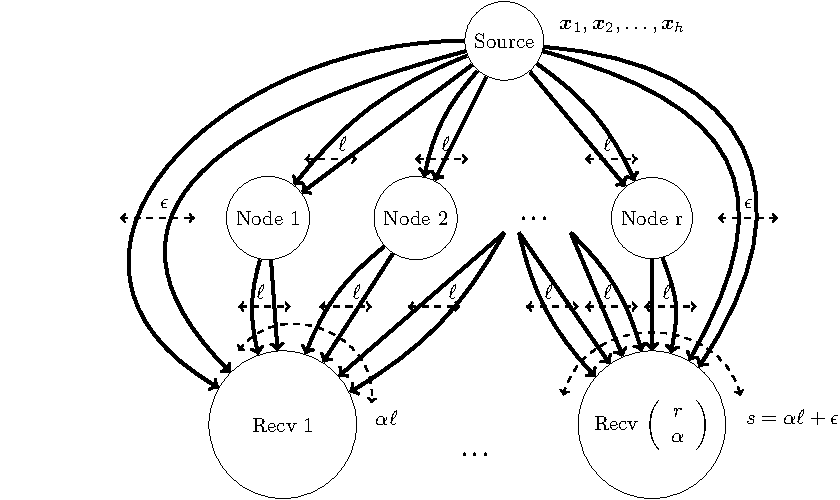
\includegraphics[width=0.5\paperwidth]{E:/Documents/TUM/THESIS/thesisCOD_Ha/figures/generalized_combination_nw}
\end{figure}

\begin{table}[H]
\caption{Parameters of network coding \label{tab:Parameters-of-network}}

\begin{tabular}{c|>{\centering}p{0.48\paperwidth}}
$h$ & The number of source messages\tabularnewline
\hline 
$r$ & The number of nodes in the middle layer\tabularnewline
\hline 
$\left(\begin{array}{c}
r\\
\alpha
\end{array}\right)$ & The number of receivers\tabularnewline
\hline 
$\ell$ & The source connects to each node by $\ell$ parallel links, and each
node also connects to one receiver by $\ell$ parallel links\tabularnewline
\hline 
$\alpha$ & A receiver is connected by any $\alpha$ nodes in the middle layer\tabularnewline
\hline 
$\epsilon$ & The source additionally connects to each receiver by $\epsilon$ direct
parallel links\tabularnewline
\hline 
$s$ & Each receiver is connected by $s$ links in total, with $s=\alpha\ell+\epsilon$.\tabularnewline
\end{tabular}
\end{table}


\section{Network Coding For This Network Family}

\subsection{Scalar network coding}

A message is equivalent to a symbol over $\ensuremath{\mathbb{F}}_{q_{s}}$.
As a network of the multicast model, all receivers request the same
packet of $h$ symbols at the same time \cite{Trautmann:2013}. A
packet is a 1-dimentional subspace of $\ensuremath{\mathbb{F}}_{q_{s}}^{h}$;
hence, each receiver must obtain a subspace of $\ensuremath{\mathbb{F}}_{q_{s}}^{h}$,
whose dimension is at least $h$, to be able to reconstruct the packet.
Through $\epsilon$ direct links connected from the source to a receiver,
the source can provide any required $\epsilon$ 1-dimensional subspaces
of $\ensuremath{\mathbb{F}}_{q_{s}}^{h}$ for the corresponding receiver.
Each receiver can accordingly reconstruct the packet if and only if
the linear span of $\alpha$ $l$-dimensional subspaces of $\ensuremath{\mathbb{F}}_{q_{s}}^{h}$
from the nodes is at least of dimension $h-\epsilon$. When this necessary
condition is satisfied, the network is said to have a \textit{solution}
or to be \textit{solvable}.
\begin{thm}
The $(0,1)-\mathcal{N}_{h,r,s}$ network has a solution if and only
if there exists an $\left(r,\left|\ensuremath{\mathbb{F}}_{q_{s}}\right|h,r-\alpha+1\right)$
$\left|\ensuremath{\mathbb{F}}_{q_{s}}\right|$-ary error correcting
code. \cite{Riis:2006}
\end{thm}
%
\begin{thm}
The $(\epsilon,l)-\mathcal{N}_{h,r,s=\alpha l+\epsilon}$network is
solvable over $\ensuremath{\mathbb{F}}_{q}$ if and only if there
exists an $\alpha-\left(h,l,h-l-\epsilon\right)_{q}^{c}$ code with
$r$ codewords. \cite{Zhang:2019} \label{theo:scalar_sol_exist}
\end{thm}

\subsection{Vector network coding}

The messages are vectors of length $t$ over $\ensuremath{\mathbb{F}}_{q}$.
Hence, a vector solution is over field size $q$ and dimension $t$.
Such a vector solution has the same alphabet size as a scalar solution
of field size $q^{t}$, and we denote $q_{v}=q^{t}$. A mapping from
the scalar solution of field size $q^{t}$ to a equivalent vector
solution is represented in Example \ref{ex:scalar_vector_mapping}.
Similarly with the scalar \textit{linear} coding solution, each receiver
can reconstruct its requested packet if and only if any $\alpha$
$\left(lt\right)$-dimensional subspaces span a subspace of dimension
at least $\left(h-\epsilon\right)t$.
\begin{thm}
A vector solution for the $(\epsilon,l)-\mathcal{N}_{h,r,s}$ network
exists if and only if there exists $\mathcal{G}_{q}\left(ht,lt\right)$
such that any $\alpha$ subspaces of the set span a subspace of dimension
at least $\left(h-\epsilon\right)t$. \cite{Zhang:2019}
\end{thm}
%
\begin{thm}
The $(\epsilon,l)-\mathcal{N}_{h,r,s=\alpha l+\epsilon}$network is
solvable with vectors of length $t$ over $\ensuremath{\mathbb{F}}_{q}$
if and only if there exists an $\alpha-\left(ht,lt,ht-lt-\epsilon t\right)_{q}^{c}$
code with $r$ codewords. \cite{Zhang:2019}
\end{thm}
\begin{cor}
The $\alpha-\left(n=ht,n-k=ht-lt,\lambda=ht-lt-\epsilon t\right)_{q}^{m}$
code formed from the dual subspaces of the $\alpha-\left(n=ht,k=lt,\lambda=ht-lt-\epsilon t\right)_{q}^{c}$
code yields the upper bound of $\mathcal{A}_{q}\left(n=ht,n-k=ht-lt,\alpha;\lambda\right)$
as maximum number of nodes for a vector network coding of the $(\epsilon,l)-\mathcal{N}_{h,r,s}$
network. \label{cor:dual_subspaces}
\end{cor}

\subsection{Network as a matrix channel}

To formulate this description, the source has a set of disjoint messages
referred to packets which are either symbols from $\ensuremath{\mathbb{F}}_{q_{s}}$
(scalar coding) or vectors of length $t$ over $\ensuremath{\mathbb{F}}_{q}$
(vector coding). Each link in the network carries functions of the
packets, and a \textit{network code} is a set of these functions.
The network code is called \textit{linear} if all the functions are
linear and nonlinear otherwise. Each receiver $R_{j},j\in\left\{ 1,\ldots,N\right\} $
requests a subset of the source's length-$h$ messages, and this subset
is called a \textit{packet}. Through all the functions on the links
from the source to each receiver, the receiver obtains several linear
combinations of the $h$ messages to form a linear system of equations
for its requested packets. The coefficients of a linear combination
are called \textit{global coding vectors}. The linear equation system
that any receiver $R_{j}$ has to solve is as following:

\begin{equation}
\begin{array}{c|c}
Scalar & Vector\\
\underset{\ensuremath{\mathbb{F}}_{q_{s}}^{s}}{\underbrace{\left[\begin{array}{c}
y_{j_{1}}\\
\vdots\\
y_{j_{s}}
\end{array}\right]}}=\underset{\ensuremath{\mathbb{F}}_{q_{s}}^{s\times h}}{\underbrace{\boldsymbol{A}_{j}}}\cdot\underset{\ensuremath{\mathbb{F}}_{q_{s}}^{h}}{\underbrace{\left[\begin{array}{c}
x_{1}\\
\vdots\\
x_{h}
\end{array}\right]}} & \underset{\ensuremath{\mathbb{F}}_{q}^{st}}{\underbrace{\left[\begin{array}{c}
\underline{y}_{j_{1}}\\
\vdots\\
\underline{y}_{j_{s}}
\end{array}\right]}}=\underset{\ensuremath{\mathbb{F}}_{q}^{st\times th}}{\underbrace{\boldsymbol{A}_{j}}}\cdot\underset{\ensuremath{\mathbb{F}}_{q}^{th}}{\underbrace{\left[\begin{array}{c}
\underline{x}_{1}\\
\vdots\\
\underline{x}_{h}
\end{array}\right]}}
\end{array}\label{eq:linear_system}
\end{equation}

The transfer matrix $\boldsymbol{A}_{j}$ contains the links' \textit{global
coding vectors}, which are combined by the coefficients of linear
combinations on $\alpha l$ links from $\alpha$ nodes and $\epsilon$
direct-links to the corresponding receiver $R_{j}$:

\[
\begin{array}{c|c}
Scalar & Vector\\
\boldsymbol{A}_{j}=\left[\begin{array}{c}
\underline{a}_{j_{1}}\\
\vdots\\
\underline{a}_{j_{\alpha l}}\\
\vdots\\
\underline{a}_{j_{\alpha l+\epsilon}}
\end{array}\right] & \boldsymbol{A}_{j}=\left[\begin{array}{c}
\boldsymbol{A}_{j_{1}}\\
\vdots\\
\boldsymbol{A}_{j_{\alpha l}}\\
\vdots\\
\boldsymbol{A}_{j_{\alpha l+\epsilon}}
\end{array}\right]
\end{array}
\]

In general, the network is represented as a matrix channel for both
scalar and vector coding:
\begin{defn}
Network As Matrix Channel

The channel output can be written as: $\boldsymbol{Y}_{j}=\boldsymbol{A}_{j}\cdot\boldsymbol{X}$
\end{defn}
Because we reconstruct $\boldsymbol{X}$ with knowing $\boldsymbol{A}_{j}$,
i.e. the network structure is known, our network is coherent. A network
is \textit{sovable} or a network code is a \textit{solution}, if each
receiver can reconstruct its requested messages or solve the system
with a unique solution for scalars $x_{1},\ldots,x_{h}$, or vectors
$\underline{x}_{1},\ldots,\underline{x}_{h}$. Therefore, we want
to find global coding vectors such that the matrix $\boldsymbol{A}_{j}$
has full-rank for every $j=1,\ldots,N$, and such that $q_{s}$ or
$q^{t}$ is minimized. In Example \ref{ex:scalar_vector_mapping},
we provide a vector solution of field size $q$ and dimension $t$,
which has the same alphabet size as a scalar solution of field size
$q^{t}$
\begin{example}
\label{ex:scalar_vector_mapping} 

Given $h=3,q=2,t=2$, we consider the extension field $\ensuremath{\mathbb{F}}_{q^{t}=2^{2}}$.
The example shows how mapping messages from scalar coding to vector
coding.
\end{example}
\begin{figure}[H]
\caption{The mapping of scalar solution over $\ensuremath{\mathbb{F}}_{q_{s}=q^{t}}$
to the equivalen vector solution\label{fig:x_mapping}}

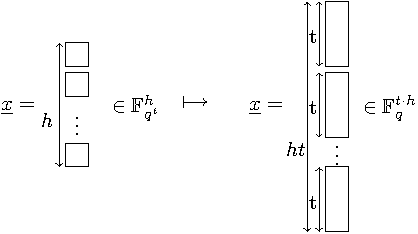
\includegraphics[width=0.3\paperwidth]{E:/Documents/TUM/THESIS/thesisCOD_Ha/figures/x_mapping}
\end{figure}

\begin{example}
We use the table of the extension field $\ensuremath{\mathbb{F}}_{2^{2}}$
with the primitive polynomial $f(x)=x^{2}+x+1$:
\end{example}
\begin{tabular}{|c|c|c|}
\hline 
power of $\alpha$ & polynomial & binary vector\tabularnewline
\hline 
- & 0 & 00\tabularnewline
\hline 
$\alpha^{0}$ & 1 & 01\tabularnewline
\hline 
$\alpha^{1}$ & $\alpha$ & 10\tabularnewline
\hline 
$\alpha^{2}$ & $\alpha+1$ & 11\tabularnewline
\hline 
\end{tabular}

For scalar coding, the messages are $x_{1},\ldots,x_{h=3}\in\ensuremath{\mathbb{F}}_{2^{2}}$
, and for vector coding the messages are $\underline{x}_{1},\ldots,\underline{x}_{h=3}\in\ensuremath{\mathbb{F}}_{2}^{2}$.
From the polynomial column, let's choose arbitrarily a scalar vector
$\underline{x}_{scalar}=(x_{1},x_{2},x_{3})=(1,\alpha,\alpha+1)$.
Then, we map it to $\underline{x}_{vector}=(\underline{x}_{1},\underline{x}_{2},\underline{x}_{3})$
by using the binary vector column as following:

\[
\left[\begin{array}{c}
x_{1}=1\\
x_{2}=\alpha\\
x_{3}=\alpha+1
\end{array}\right]\mapsto\left[\begin{array}{c}
\left(\begin{array}{c}
1\\
0
\end{array}\right)\\
\left(\begin{array}{c}
0\\
1
\end{array}\right)\\
\left(\begin{array}{c}
1\\
1
\end{array}\right)
\end{array}\right],
\]

where we use the following rule for mapping $x_{i}$ individually:
$a_{0}\cdot\alpha^{0}+a_{1}\cdot\alpha^{1}+\ldots+a_{t-1}\cdot\alpha^{t-1}\mapsto\left(\begin{array}{c}
a_{0}\\
a_{1}\\
\vdots\\
a_{t-1}
\end{array}\right)$.

To summarize the notations of both scalar and vector coding, we represent
them in the Table~\ref{tab:notations}:

\begin{table}[H]
\caption{Notations of network coding}

\label{tab:notations} 

\begin{tabular}{|>{\centering}p{0.2\paperwidth}|c|c|}
\hline 
 & Scalar Coding & Vector coding\tabularnewline
\hline 
\hline 
Source Messages/Packets & $\begin{array}{c}
x_{1},\ldots,x_{h}\in\ensuremath{\mathbb{F}}_{q_{s}}\\
\underline{x}\in\ensuremath{\mathbb{F}}_{q_{s}}^{h}
\end{array}$ & $\begin{array}{c}
\underline{x}_{1},\ldots,\underline{x}_{h}\in\ensuremath{\mathbb{F}}_{q}^{t}\\
\underline{x}\in\ensuremath{\mathbb{F}}_{q}^{th}
\end{array}$\tabularnewline
\hline 
Global Coding Vectors Of Receiver $R_{j}$ & $\underline{a}_{j_{1}},\ldots,\underline{a}_{j_{s}}\in\ensuremath{\mathbb{F}}_{q_{s}}^{h}$ & $\boldsymbol{A}_{j_{1}},\ldots,\boldsymbol{A}_{j_{s}}\in\ensuremath{\mathbb{F}}_{q}^{t\times th}$\tabularnewline
\hline 
Transfer Matrix Of Receiver $R_{j}$ & $\boldsymbol{A}_{j}\in\ensuremath{\mathbb{F}}_{q^{t}}^{s\times h}$ & $\boldsymbol{A}_{j}\in\ensuremath{\mathbb{F}}_{q}^{st\times th}$\tabularnewline
\hline 
Packets On Receiver $R_{j}$ & $\begin{array}{c}
y_{j_{1}},\ldots,y_{j_{s}}\in\ensuremath{\mathbb{F}}_{q_{s}}\\
\underline{y}\in\ensuremath{\mathbb{F}}_{q_{s}}^{s}
\end{array}$ & $\begin{array}{c}
\underline{y}_{j_{1}},\ldots,\underline{y}_{j_{s}}\in\ensuremath{\mathbb{F}}_{q}^{t}\\
\boldsymbol{Y}_{j}\in\ensuremath{\mathbb{F}}_{q}^{st}
\end{array}$\tabularnewline
\hline 
Number of nodes & $r_{scalar}$ & $r_{vector}$\tabularnewline
\hline 
\end{tabular}
\end{table}

\begin{rem}
By using the vector coding, the upper bound number of solutions increases
from $q^{tkh}$ to $q^{t^{2}kh}$. Therefore, vector network coding
offers more freedom in choosing the coding coefficients than does
scalar linear coding for equivalent alphabet sizes, and a smaller
alphabet size might be achievable \cite{Ebrahimi2011}. By this advantage,
we can have higher amount of receivers, i.e. higher amount of nodes,
in vector network coding.
\end{rem}

\subsection{Comparison between scalar and vector solutions by the gap size}

The \textit{gap} represents the difference between the smallest field
(alphabet) size for which a scalar linear solution exists and the
smallest alphatbet size for which we can construct a vector solution.
In this study, we define a solvable vector network coding over the
field size $\ensuremath{\mathbb{F}}_{q}^{t}$, and we conjecture the
minimum amount of nodes such vector solution can achieve, i.e. $r_{vector}\geq f_{1}(q)$,
with $f_{1}:\mathbb{Z}\mapsto\mathbb{Z}$. Meanwhile, we has a scalar
solution for the same network existing if and only if: $r_{scalar}\leq f_{2}\left(q_{s}\right)$,
with $f_{2}:\mathbb{Z}\mapsto\mathbb{Z}$. To find the field size
$q_{s}$ required for a scalar solution to reach the minimum achievable
vector solution's nodes in this setting, we consider $r_{max,scalar}=f_{2}\left(q_{s}\right)=f_{1}(q)=r_{min,vector}$.
Finally, we calculate the gap by $g=q_{s}-q_{v}=q_{s}-q^{t}.$ Throughout
this study, we show that vectors solutions significantly reduce the
required alphabet size by this gap. 

\section{Special cases of generalized combination network}

\subsection{The $(l-1)$-Direct Links and $l$-Parrallel Links $\mathcal{N}_{h=2l,r,s=3l-1}$}

This subfamily contains the largest number of direct links from the
source to the receivers. For $l\geq2$, this network $\left(\epsilon=l-1,l\right)-\mathcal{N}_{h=2l,r,s=3l-1}$
yields the gap $q^{(l-1)t^{2}/l+\mathcal{O}(t)}$ between vector solutions
and optimal scalar solutions. The vector solution is based on an $\mathcal{MRD}\left[lt\times lt,t\right]_{q}$
code. Further, the gap tends to $q^{t^{2}/2+\mathcal{O}(t)}$ for
large $l$.
\begin{lem}
There is a scalar linear solution of field size $q_{s}$ for the $\left(\epsilon=l-1,l\right)-\mathcal{N}_{h=2l,r,s=3l-1}$
network, where $l\geq2$, if and only if $r\leq\left[\begin{array}{c}
2l\\
l
\end{array}\right]_{q_{s}}$.
\end{lem}

\subsection{The 1-Direct Link and $l$-Parrallel Links $\mathcal{N}_{h=2l,r,s=2l+1}$}

This is the smallest direct-link subfamily has an vector solution
outperforming the optimal scalar solution, i.e. an vector solution
outperforming the optimal scalar has not yet been found for the network
$(0,l>1)-\mathcal{N}_{h,r,s}$. Similar to the previous subfamily
$\left(\epsilon=l-1,l\right)-\mathcal{N}_{h=2l,r,s=3l-1}$, when $l\geq2$
or $h\geq4$, this network yields the largest gap $q^{t^{2}/2+\mathcal{O}(t)}$
in the alphabet size by using the same approach with an $\mathcal{MRD}\left[lt\times lt,(l-1)t\right]_{q}$
code. 

\subsection{The $\epsilon$-Direct Links $\mathcal{N}_{h,r,s}$}

This subfamily is denoted as $\left(\epsilon\geq1,l=1\right)-\mathcal{N}_{h,r,s}$
and is the most focus topic on this thesis, because it motivates some
interesting questions on a classic coding problem and on a new type
of subspace code problem. In the chapter 3, we show our largest code
set with low number of subspace codes for the network $\left(\epsilon=1,l=1\right)-\mathcal{N}_{h=3,r,s=4}$.

\subsection{The $\left(\epsilon=0,l=1\right)-\mathcal{N}_{h,r,s}$ Combination
Network}

Since the scalar solution for the combination network uses an $MDS$
code, a vector solution based on subspace codes must go beyond the
$MDS$ bound, i.e. Singleton bound $d\leq n-k+1$, to outperform the
scalar one. In paper \cite{Wachter-Zeh:2018}, it is proved that vector
solutions based on subspace codes cannot outperform optimal scalar
linear solutions for $h=2$, and they conjecture it for all $h$.
Unfortunately, a vector solution based on an $\mathcal{MRD}\left[t\times t,t\right]_{q}$
code is also proved that it cannot outperform the optimal scalar linear
solution.

\subsection{The 2 networks yields gap $q^{(h-3)t^{2}/(h-1)+\mathcal{O}(t)}$}

For $h=2l-1$: $\left(\epsilon=l-2,l\right)-\mathcal{N}_{h=2l-1,r,s=3l-2}$

For $h=2l+1$: $\left(\epsilon=l-1,l\right)-\mathcal{N}_{h=2l+1,r,s=3l-1}$

\part{Combinatorial Results}

In previous studies \cite{Wachter-Zeh:2018}, there was no general
vector solution found for multicast networks with $h=3$ messages.
Hence, we start with a probabilistic argument to prove that there
exists a vector solution outperforming the optimal linear solution
for the $\left(\epsilon=1,l=1\right)-\mathcal{N}_{h=3,r,s=4}$ network.
Then we generalize the proof to the $\left(\epsilon=1,l=1\right)-\mathcal{N}_{h,r,s}$
network.

\section{$\left(\epsilon=1,l=1\right)-\mathcal{N}_{h=3,r,s=4}$ Network}

\begin{figure}[H]
\caption{The $(\epsilon=1,l=1)-\mathcal{N}_{h=3,r,s=4}$ network\label{fig:nw_e1_l1_h3_r_s4}}

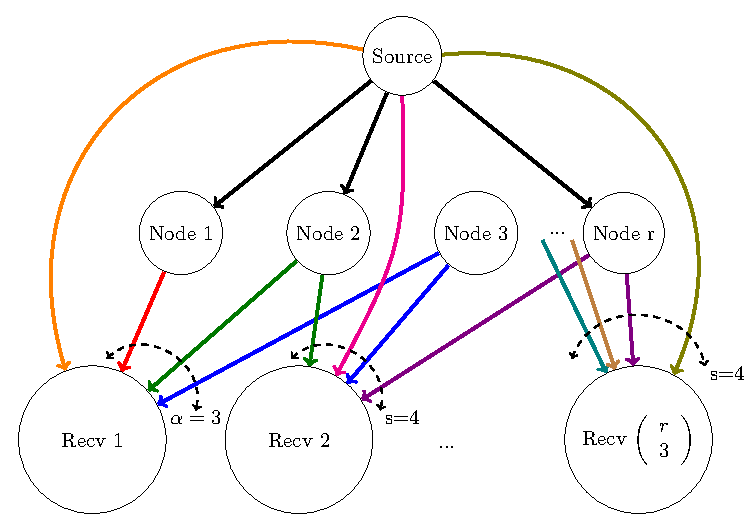
\includegraphics[width=0.5\paperwidth]{E:/Documents/TUM/THESIS/thesisCOD_Ha/figures/nw_e1_l1_h3_r_s4}
\end{figure}

\begin{conjecture}
For the network $\left(\epsilon=1,l=1\right)-\mathcal{N}_{h=3,r,s=4}$,
the probability that vector solution does not exist is less than or
equal to $\stackrel[i=0]{2t-1}{\mathop{\sum}}\frac{\stackrel[j=0]{i-1}{\mathop{\prod}}\frac{\left(q^{3t}-q^{j}\right)^{2}}{q^{i}-q^{j}}}{q^{9t^{2}}}$.
\end{conjecture}
\textit{Proof:} Following to Equation \ref{eq:linear_system}, each
receiver must solve a linear equation system of 3 variables with 4
equations to recover $h=3$ messages as below:

\[
\left[\begin{array}{c}
\underline{y}_{j_{1}}\\
\underline{y}_{j_{2}}\\
\underline{y}_{j_{3}}\\
\underline{y}_{j_{4}}
\end{array}\right]=\left[\begin{array}{c}
\boldsymbol{A}_{j_{1}}\\
\boldsymbol{A}_{j_{2}}\\
\boldsymbol{A}_{j_{3}}\\
\boldsymbol{A}_{j_{4}}
\end{array}\right]\cdot\left[\begin{array}{c}
\underline{x}_{1}\\
\underline{x}_{2}\\
\underline{x}_{3}
\end{array}\right],
\]

with $\underline{x}_{i},\underline{y}_{j_{v}}\in\ensuremath{\mathbb{F}}_{q}^{t},\boldsymbol{A}_{j_{v}}\in\ensuremath{\mathbb{F}}_{q}^{t\times3t}$
for $v=1,\ldots,4$, and $\boldsymbol{A}_{j_{1}},\ldots,\boldsymbol{A}_{j_{3}}$
must be distinct.

The network is solvable, if $\boldsymbol{A}_{j}$ has full-rank for
every $j=1,\ldots,N$, i.e. $\boldsymbol{A}_{j_{v}}$ must satisfy:

\[
rk\left[\begin{array}{c}
\boldsymbol{A}_{j_{1}}\\
\boldsymbol{A}_{j_{2}}\\
\boldsymbol{A}_{j_{3}}\\
\boldsymbol{A}_{j_{4}}
\end{array}\right]\geq3t
\]

In order to satisfy $rk\left[\boldsymbol{A}_{j}\right]\geq3t$, we
can easily choose suitable values for the coefficient $\boldsymbol{A}_{j}^{(4)}$
on the direct link from the source to $R_{j}$. However, the coefficients
on the links from nodes to receivers are matters. Therefore, we focus
on the following requirement:

\begin{equation}
rk\left[\begin{array}{c}
\boldsymbol{A}_{j_{1}}\\
\boldsymbol{A}_{j_{2}}\\
\boldsymbol{A}_{j_{3}}
\end{array}\right]\geq2t\label{eq:rk_rqm_e1l1h3s4}
\end{equation}

Therefore, $rk\left[\begin{array}{c}
\boldsymbol{A}_{j_{1}}\\
\boldsymbol{A}_{j_{2}}\\
\boldsymbol{A}_{j_{3}}
\end{array}\right]\geq2t$ implies $rk\left[\boldsymbol{A}_{j}\right]\geq3t$, or to satisfy
$rk\left[\boldsymbol{A}_{j}\right]\geq3t$, we need $rk\left[\begin{array}{c}
\boldsymbol{A}_{j_{1}}\\
\boldsymbol{A}_{j_{2}}\\
\boldsymbol{A}_{j_{3}}
\end{array}\right]\geq2t$. In Section \ref{sec:Description_GCN}, we have $N=\left(\begin{array}{c}
r\\
\alpha
\end{array}\right)$ and $\alpha=3$ as a fixed values. Therefore, maximizing the number
of receivers is equivalent to maximize $r$ under the constraint \ref{eq:rk_rqm_e1l1h3s4}.
$\boldsymbol{A}_{j_{1}},\boldsymbol{A}_{j_{2}},\boldsymbol{A}_{j_{3}}$
are matrices formed on any 3 of $r$ links from nodes to receivers,
i.e. these 3 matrices are randomly chosen from a set of $r$ matrices.
We formalize the problem by an approach with Lov\'asz local lemma
\cite{MosheSchwartz:2018}.
\begin{thm}[Symmetric Lov\'asz local lemma (LLL)]
\label{thm:LLL} \cite{Schwarz:2013}

A set of events $\mathcal{E}_{i}$, with $i=1,\ldots,n$, such that
each event occurs with probability at most $p$. If each event is
independent of all others except for at most $d$ of them and $4dp\leq1$,
then:

\[
Pr\left[\stackrel[i=1]{n}{\bigcap}\overline{\mathcal{E}}_{i}\right]>0
\]
\end{thm}
For our problem, let $\mathcal{E}_{i}$ denote the following event:

\[
Pr\left[\mathcal{E}_{i}\right]=Pr\left[rk\left[\begin{array}{c}
\boldsymbol{A}_{j_{1}}\\
\boldsymbol{A}_{j_{2}}\\
\boldsymbol{A}_{j_{3}}
\end{array}\right]<2t\right]
\]

Because the requirement on rank is opposite, we consider the complement
event $T$:

\[
rk\left[\begin{array}{c}
\boldsymbol{A}_{j_{1}}\\
\boldsymbol{A}_{j_{2}}\\
\boldsymbol{A}_{j_{3}}
\end{array}\right]\geq2t,\forall1\leq j_{1}<j_{2}<j_{3}\leq r
\]

By the intersection rule, we have:

\[
T=\underset{\mathcal{E}_{i}\in\mathcal{E}}{\bigcap}\overline{\mathcal{E}}_{i}
\]

The probability of event $T$ indicates a measure quantifying the
likelihood that we will be able to construct $rk\left[\boldsymbol{A}_{j}\right]\geq3t$
with $j_{1,}j_{2},j_{3}$ in the integer numbers between $1$ and
$r$, including both. We need to maximize $r$, but the rank requirement
is still satisfied, i.e. the probabilty must be higher than $0$:

\begin{eqnarray*}
 & Pr\left[rk\left[\begin{array}{c}
\boldsymbol{A}_{j_{1}}\\
\boldsymbol{A}_{j_{2}}\\
\boldsymbol{A}_{j_{3}}
\end{array}\right]\geq2t,\forall1\leq j_{1}<j_{2}<j_{3}\leq r\right] & >0\\
\Leftrightarrow & Pr\left[T\right] & >0\\
\Leftrightarrow & Pr\left[\underset{\mathcal{E}_{i}\in\mathcal{E}}{\bigcap}\overline{\mathcal{E}}_{i}\right] & >0
\end{eqnarray*}

Following to LLL, each event occurst with probability at most $p$:

\[
Pr\left[\mathcal{E}_{i}\right]=Pr\left[rk\left[\begin{array}{c}
\boldsymbol{A}_{i_{1}}\\
\boldsymbol{A}_{i_{2}}\\
\boldsymbol{A}_{i_{3}}
\end{array}\right]<2t\right]\leq p
\]

Regarding to the left-hand side:

\begin{eqnarray}
Pr\left[rk\left[\begin{array}{c}
\boldsymbol{A}_{i_{1}}\\
\boldsymbol{A}_{i_{2}}\\
\boldsymbol{A}_{i_{3}}
\end{array}\right]<2t\right] & = & \stackrel[i=0]{2t-1}{\mathop{\sum}}Pr\left[rk\left[\begin{array}{c}
\boldsymbol{A}_{i_{1}}\\
\boldsymbol{A}_{i_{2}}\\
\boldsymbol{A}_{i_{3}}
\end{array}\right]=i\right]\nonumber \\
 & \overset{1}{=} & \stackrel[i=0]{2t-1}{\mathop{\sum}}\frac{N_{t,m,n}}{q^{m\cdot n}}\nonumber \\
 & = & \stackrel[i=0]{2t-1}{\mathop{\sum}}\frac{\stackrel[j=0]{i-1}{\mathop{\prod}}\frac{\left(q^{m}-q^{j}\right)\left(q^{n}-q^{j}\right)}{q^{i}-q^{j}}}{q^{m\cdot n}}\nonumber \\
 & \overset{2}{=} & \stackrel[i=0]{2t-1}{\mathop{\sum}}\frac{\stackrel[j=0]{i-1}{\mathop{\prod}}\frac{\left(q^{3t}-q^{j}\right)^{2}}{q^{i}-q^{j}}}{q^{9t^{2}}}\Square\label{eq:p_eq_h3}
\end{eqnarray}

By varying $t$ in Equation (\ref{eq:p_eq_h3}), we have the following
table:

\begin{table}[H]
\caption{$r$ over variations of t\label{tab:r_over_t}}

\begin{tabular}{|c|c|c|}
\hline 
t & Scalar Solution & Vector Solution\tabularnewline
\hline 
\hline 
1 & $r_{scalar}\leq14$ & $r_{vector}\geq3$\tabularnewline
\hline 
2 & $r_{scalar}\leq42$ & $r_{vector}\geq7\,\left(67^{*},\,89^{**}\right)$\tabularnewline
\hline 
3 & $r_{scalar}\leq146$ & $r_{vector}\geq62\,\left(166^{*}\right)$ \tabularnewline
\hline 
4 & $r_{scalar}\leq546$ & $r_{vector}\geq1317$\tabularnewline
\hline 
5 & $r_{scalar}\leq2114$ & $r_{vector}\geq58472$\tabularnewline
\hline 
6 & $r_{scalar}\leq8322$ & $r_{vector}>10^{6}$\tabularnewline
\hline 
\end{tabular}

{*}, {*}{*}: computational results in construction 1 and construction
2 respectively
\end{table}

In the table (\ref{tab:r_over_t}), the vector solution outperforms
the scalar solution when $t\geq4$ for the network $\left(\epsilon=1,l=1\right)-\ensuremath{N}_{h=3,r,s=4}$.
This is sufficient, later on we show computational results which vector
solutions outperform scalar solutions in case of $t=2$ and $t=3$.
\begin{conjecture}
For the network $\left(\epsilon=1,l=1\right)-\mathcal{N}_{h=3,r,s=4}$,
the achieved gap is $q^{t^{2}/4+\mathcal{O}(t)}$.
\end{conjecture}
\textit{Proof:} We proceed the other constraint of LLL: $4dp\leq1$.
Regarding to $d$, we have:

\begin{eqnarray*}
d(r) & \leq & 3\cdot\left(\begin{array}{c}
r-1\\
2
\end{array}\right)=3\cdot\frac{\left(r-1\right)\left(r-2\right)}{2}=\frac{3}{2}\left(r^{2}-3r+2\right)=d_{1}(r)\\
 & \leq & \frac{3}{2}r^{2}=d_{2}(r)
\end{eqnarray*}

Hence, we have below implications:

\begin{eqnarray*}
 & 4\cdot p\cdot d_{2}(r) & \leq1\\
\overset{1}{\Rightarrow} & 4\cdot p\cdot d_{1}(r) & \leq1\\
\overset{2}{\Rightarrow} & 4\cdot p\cdot d(r) & \leq1
\end{eqnarray*}

1: $d_{1}(r)\leq d_{2}(r)$

2: $d(r)\leq d_{1}(r)$

In consideration of $d_{2}(r)$:

\[
4\cdot p\cdot d_{2}(r)\leq1\Rightarrow4\cdot p\cdot\frac{3}{2}r^{2}\leq1\Rightarrow r\leq\sqrt{\frac{1}{6p}}=r_{min,vector}
\]

\begin{figure}[H]
\caption{The vector network coding of $(\epsilon=1,l=1)-\mathcal{N}_{h=3,r,s=4}$
represents as a matrix problem\label{fig:rk_h3}}

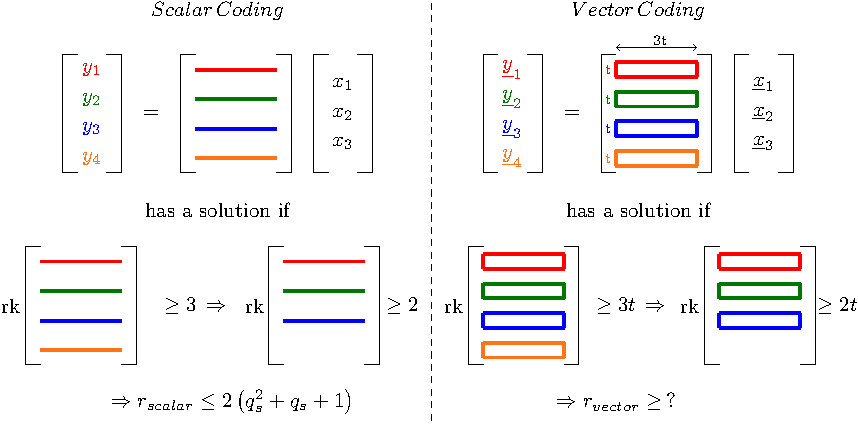
\includegraphics[width=0.5\paperwidth]{E:/Documents/TUM/THESIS/thesisCOD_Ha/figures/rk_h3}
\end{figure}

Similarly with above, $d$ and $r$ are propotional, so minimizing
$r$ is equivelent to maximizing $p$. The purpose is to achieve a
strict lower bound proving vector solutions always outperform scalar
solutions in a specific range of $t$, i.e., $r_{max}$asymptotes
to a value higher than $r_{scalar}$. Now, we begin to maximize $p$.
We consider the nominator of Equation (\ref{eq:p_eq_h3}):

\[
\stackrel[j=0]{i-1}{\mathop{\prod}}\frac{\left(q^{3t}-q^{j}\right)^{2}}{q^{i}-q^{j}}=\frac{p_{N}^{(i)}(q)}{p_{D}^{(i)}(q)}=p^{(i)}(q)
\]

Due to $i$-times product and large $t$:

\[
\left.\begin{array}{c}
deg\left(p_{N}^{(i)}(q)\right)=q^{i6t}\\
deg\left(p_{D}^{(i)}(q)\right)=q^{i^{2}}
\end{array}\right\} \Rightarrow p^{(i)}(q)\approx q^{i6t-i^{2}}
\]

Then we have:

\[
\stackrel[i=1]{2t-1}{\mathop{\sum}}\stackrel[j=0]{i-1}{\mathop{\prod}}\frac{\left(q^{3t}-q^{j}\right)^{2}}{q^{i}-q^{j}}=\stackrel[i=1]{2t-1}{\mathop{\sum}}p^{(i)}(q)\approx\stackrel[i=1]{2t-1}{\mathop{\sum}}q^{i6t-i^{2}}
\]

To maximize the sum, we set derivation of to 0 and find its root:

\begin{eqnarray*}
 & \left(i6t-i^{2}\right)^{'} & =0\\
\Leftrightarrow & 6t-2i & =0\\
\Leftrightarrow & i & =3t
\end{eqnarray*}

However, the upper limit of sum is $\left(2t-1\right)$, which is
less than $3t$.

\[
\Rightarrow max\left\{ q^{i6t-i^{2}}:i=1,2\ldots,2t-1\right\} =\left.q^{i6t-i^{2}}\right|_{i=2t-1}=q^{8t^{2}-2t-1}
\]

Hence, by using the exact bound $\Theta$, we have:

\[
\stackrel[i=1]{2t-1}{\mathop{\sum}}p^{(i)}(q)\in\Theta\left(max\left\{ q^{i6t-i^{2}}:i=1,2\ldots,2t-1\right\} \right)=\Theta\left(q^{8t^{2}-2t-1}\right)
\]

\[
\Rightarrow\frac{1+\stackrel[i=1]{2t-1}{\mathop{\sum}}p^{(i)}(q)}{q^{9t^{2}}}\approx\frac{\stackrel[i=1]{2t-1}{\mathop{\sum}}p^{(i)}(q)}{q^{9t^{2}}}\in\Theta\left(q^{-t^{2}-2t-1}\right)
\]

Finally, we have:

\[
r_{min,vector}\in\Omega\left(\sqrt{\frac{1}{6p}}\right)=\Omega\left(\sqrt{\frac{1}{6q^{-t^{2}-2t-1}}}\right)=\Omega\left(q^{t^{2}/2+\mathcal{O}\left(t\right)}\right)
\]

Further we have: $r_{max,scalar}\in\mathcal{O}\left(q_{s}^{2}\right)$
\cite{Wachter-Zeh:2018}, specifically, 
\begin{equation}
r_{scalar}\leq2\left[\begin{array}{c}
3\\
1
\end{array}\right]_{q_{s}}=2\left(q_{s}^{2}+q_{s}+1\right)\label{eq:r_scalar_max}
\end{equation}
. 

We have the gap size:

\begin{eqnarray*}
 & r_{max,scalar} & =r_{min,vector}\\
\Leftrightarrow & q_{s}^{2} & =q^{t^{2}/2+\mathcal{O}(t)}\\
\Leftrightarrow & q_{s} & ^{=}q^{t^{2}/4+\mathcal{O}(t)}\\
\Rightarrow & g & =q_{s}-q_{v}=q^{t^{2}/4+\mathcal{O}(t)}\Square
\end{eqnarray*}


\section{$\left(\epsilon=1,l=1\right)-\mathcal{N}_{h,r,s}$ Network}

\subsection{Find the lower bound of $r_{max,vector}$}

Following to Theorem (\ref{nw_parameters}), we are interested in
the following range: $l+\epsilon+1\leq h\leq\alpha l+\epsilon$.

As previous, $\boldsymbol{A}_{j_{1}},\ldots,\boldsymbol{A}_{j_{h-\epsilon}}\in\ensuremath{\mathbb{F}}_{q}^{t\times ht}$
and we need to satisfy the following:

\[
rk\left[\begin{array}{c}
\boldsymbol{A}_{j_{1}}\\
\vdots\\
\boldsymbol{A}_{j_{h-\epsilon}}
\end{array}\right]\geq ht-t\Leftrightarrow rk\left[\boldsymbol{A}_{j}\right]\geq(h-1)t
\]

We can formulate it by the following coding problem in Grassmannian:

\noindent\fbox{\begin{minipage}[t]{1\columnwidth - 2\fboxsep - 2\fboxrule}%
Find the largest set of subspaces from $\mathcal{G}_{q}\left(ht,t\right)$
such that any $\alpha$ subspaces of the set span a subspace of dimension
at least $\left(h-1\right)t$.%
\end{minipage}}

Similar to $\left(\epsilon=1,l=1\right)-\ensuremath{N}_{3,r,4}$,
we consider $p$ to proceed LLL:

\[
Pr\left[rk\left[\boldsymbol{A}\right]<(h-1)t\right]\leq p
\]

Regarding to the left-hand side:

\begin{eqnarray}
Pr\left[rk\left[\boldsymbol{A}\right]<(h-1)t\right] & = & \stackrel[i=0]{(h-1)t-1}{\mathop{\sum}}Pr\left[rk\left[\boldsymbol{A}\right]=i\right]\nonumber \\
 & \overset{1}{=} & \stackrel[i=0]{(h-1)t-1}{\mathop{\sum}}\frac{N_{i,\alpha t,ht}}{q^{\left(\alpha t\right)\left(ht\right)}}\nonumber \\
 & = & \frac{1}{q^{\left(\alpha h\right)t^{2}}}\cdot\stackrel[i=0]{(h-1)t-1}{\mathop{\sum}}\stackrel[j=0]{i-1}{\mathop{\prod}}\frac{\left(q^{\alpha t}-q^{j}\right)\left(q^{ht}-q^{j}\right)}{q^{i}-q^{j}}\label{eq:general_nw_calc_p}
\end{eqnarray}

Firstly, we consider the product:

\[
\stackrel[j=0]{i-1}{\mathop{\prod}}\frac{\left(q^{\alpha t}-q^{j}\right)\left(q^{ht}-q^{j}\right)}{q^{i}-q^{j}}=\frac{p_{N}^{(i)}(q)}{p_{D}^{(i)}(q)}=p^{(i)}(q)
\]

For $t\rightarrow\infty$:

\[
\left.\begin{array}{c}
deg\left(p_{N}^{(i)}(q)\right)=q^{i(\alpha t+ht)}\\
deg\left(p_{D}^{(i)}(q)\right)=q^{i^{2}}
\end{array}\right\} \Rightarrow p^{(i)}(q)\approx q^{i(\alpha t+ht)-i^{2}}
\]

Now, we exaluate $f(i)=i(\alpha t+ht)-i^{2}$ to find its maximum
point:

$\dot{f}(i^{*})=0\Leftrightarrow(\alpha t+ht)-2i^{*}=0\Leftrightarrow i^{*}=\frac{\alpha t+ht}{2}$

We then check whether this point within the range $i=0,\ldots,(h-1)t-1$
as following: $0\leq\frac{\alpha t+ht}{2}\leq(h-1)t-1$

With regards to the lower bound: $0\leq\frac{\alpha t+ht}{2}\Leftrightarrow t\geq\frac{2}{\alpha+h}$,
which is always true due to the given $t\geq2$ and $\alpha,h\geq3$.

Regarding to the upper bound: $\frac{\alpha t+ht}{2}\leq(h-1)t-1\Leftrightarrow t\leq\frac{-2}{\alpha+2-h}$
with $\alpha+2>h$ due to the given $\alpha l+\epsilon=\alpha+1\geq h$.
This cannot happen because of $t\geq2$, i.e. this maximum point is
over then upper-range limit.

\begin{eqnarray*}
\Rightarrow & max\left\{ q^{i(\alpha t+ht)-i^{2}}:i=1,\ldots,(h-1)t-1\right\}  & =\left.q^{i(\alpha t+ht)-i^{2}}\right|_{i=(h-1)t-1}\\
 &  & =q^{\left[\left(h-1\right)\left(\alpha+1\right)\right]t^{2}-\left(\alpha-h+2\right)t-1}
\end{eqnarray*}

Secondly, we apply the maximum value with the sum, we have:

\[
\stackrel[i=0]{(h-1)t-1}{\mathop{\sum}}p^{(i)}(q)\in\Theta\left(q^{\left[\left(h-1\right)\left(\alpha+1\right)\right]t^{2}+\mathcal{O}(t)}\right)
\]

Thirdly, we consider the 3rd requirement of LLL to figure out a lower
bound on $r_{max}$:

$d\leq\alpha\left(\begin{array}{c}
r-1\\
\alpha-1
\end{array}\right)=\alpha\frac{\left(r-1\right)\ldots\left(r-\alpha+1\right)}{\left(\alpha-1\right)!}\leq\frac{\alpha}{\left(\alpha-1\right)!}r^{^{\alpha-1}}=d_{2}$

We need $4dp\leq1$, which is satisfied if $4d_{2}p\leq1$. Therefore,
we consider:

$\frac{\alpha}{\left(\alpha-1\right)!}r^{^{\alpha-1}}\leq\frac{1}{4p}\Leftrightarrow r\leq\left(\frac{\left(\alpha-1\right)!}{4\alpha}\cdot\frac{1}{p}\right)^{\frac{1}{\alpha-1}}$

Finally, we have from above:

\begin{eqnarray*}
p & \in & \Theta\left(\frac{q^{\left[\left(h-1\right)\left(\alpha+1\right)\right]t^{2}+\mathcal{O}(t)}}{q^{\left(\alpha h\right)t^{2}}}\right)\\
\Rightarrow r_{min,vector} & \in & \Omega\left(q^{\frac{h-\alpha-1}{1-\alpha}t^{2}+\mathcal{O}(t)}\right)
\end{eqnarray*}


\subsection{Find the upper bound of $r_{max,scalar}$}

\noindent\fbox{\begin{minipage}[t]{1\columnwidth - 2\fboxsep - 2\fboxrule}%
Find $\left(\alpha+1\right)$ received vectors that span a subspace
of dimension $h$. This implies that the $\alpha$ links from the
middle layer carry $\alpha$ vectors which span a subspace of $\ensuremath{\mathbb{F}}_{q_{s}}^{h}$
whose dimension is at least $\left(h-1\right)$, with $q_{s}=q^{t}$.%
\end{minipage}}

For $3\leq\alpha<h$: all $\alpha$ links must be distinct $\Rightarrow r\leq\left[\begin{array}{c}
\alpha\\
1
\end{array}\right]_{q_{s}}\Rightarrow r\leq$

For $\alpha\geq h\geq3$: to achieve $(h-1)$-subspaces of $\ensuremath{\mathbb{F}}_{q_{s}}^{h}$,
no $\alpha$ links will contain a vector which is contained in the
same $(h-2)$-subspace.

Hence,

\[
r_{max,scalar}\leq\left(\alpha-1\right)\left[\begin{array}{c}
\alpha\\
h-2
\end{array}\right]_{q_{s}}\Rightarrow r_{max,scalar}\in\mathcal{O}\left(q_{s}^{\left(\alpha-h+2\right)\left(h-2\right)t^{2}}\right)
\]


\subsection{Calculate the gap of size}

\begin{eqnarray*}
 & r_{max,scalar} & =r_{min,vector}\\
\Leftrightarrow & q_{s}^{\left(\alpha-h+2\right)\left(h-2\right)t^{2}} & =q^{\frac{h-\alpha-1}{1-\alpha}t^{2}+\mathcal{O}(t)}\\
\Leftrightarrow & q_{s} & ^{=}q^{\frac{\alpha-h+1}{\left(\alpha-1\right)\left(\alpha-h+2\right)\left(h-2\right)}t^{2}+\mathcal{O}(t)}\\
\Rightarrow & g & =q_{s}-q_{v}=q^{\frac{\alpha-h+1}{\left(\alpha-1\right)\left(\alpha-h+2\right)\left(h-2\right)}t^{2}+\mathcal{O}(t)}\Square
\end{eqnarray*}


\part{Computational Results}

In Table \ref{tab:r_over_t}, our vector solutions are computed by
Algorithm \ref{alg:Increasing-Method} for the $\left(\epsilon=1,l=1\right)-\ensuremath{N}_{3,r,4}$
network regarding to $t=2$ and $t=3$. Both construction 1 and 2
provide better results than scalar solutions. 

Construction 1: $\begin{array}{c|c}
\boldsymbol{I}_{t} & \boldsymbol{T}\end{array}$, with $\boldsymbol{T}\in\ensuremath{\mathbb{F}}_{q}^{t\times t\left(h-1\right)}$

Construction 2: $\boldsymbol{T}\in MatrixSpaceUrs\left(t,3t\right)$

Regarding to $t=2$, for a scalar network coding solution we need
a $3-\left(3,1,1\right)_{4}^{c}$ code ($q_{v}=2^{2})$ by Theorem
\ref{theo:scalar_sol_exist}. The largest such code consists of the
21 $1$-dimensionall subspaces of $\ensuremath{\mathbb{F}}_{4}^{3}$,
each one is contained twice in the code. Therefore, the number of
nodes can be at most 42 for a scalar linear coding solution, while
for vector network coding 89 nodes can be used, i..e. $\mathcal{A}_{q=2}\left(n=6,k=4,t=3;\lambda=2\right)\geq89$
following to Corollary \ref{cor:dual_subspaces}. This is a new lower
bound for $\mathcal{A}_{2}\left(6,4,3;2\right)$ compared to a code
with 51 codewords presented in \cite{Wachter-Zeh:2018}. The smallest
alphabet size for a scalar solution with 89 nodes exists is $q_{s}=8$.
By Equation \ref{eq:r_scalar_max}, there are 73 $1$-dimensional
subspaces of $\ensuremath{\mathbb{F}}_{8}^{3}$, and each one can
be used twice in the code; therefore, we have in total 146 possible
codesword, but only 89 codewords are required.
\begin{defn}[G3]
 Let $\boldsymbol{A},\boldsymbol{B},\boldsymbol{C}\in\ensuremath{\mathbb{F}}_{q}^{n\times m}$.
Then a set $\left\{ \boldsymbol{A},\boldsymbol{B},\boldsymbol{C}\right\} $
forms a subset of $g3$ if

\[
rk\left[\begin{array}{c}
\boldsymbol{A}\\
\boldsymbol{B}\\
\boldsymbol{C}
\end{array}\right]\geq2n
\]

In other words, all $\left\{ \boldsymbol{A},\boldsymbol{B},\boldsymbol{C}\right\} $
span a subspace of $\ensuremath{\mathbb{F}}_{q}^{2n}$ whose dimension
is at least $2n$. We denote $g3_{i}$ as a subset of $g3$:

\[
g3=\left\{ \left\{ \boldsymbol{A},\boldsymbol{B},\boldsymbol{C}\right\} _{i}\right\} =\left\{ g3_{i}\right\} ,i=0,1,2,...,\left|g3\right|-1
\]

with $g3_{i}=\left\{ \boldsymbol{A},\boldsymbol{B},\boldsymbol{C}\right\} _{i}$
\end{defn}
%
\begin{defn}[Relative]
 Let $\boldsymbol{A},\boldsymbol{B},\boldsymbol{C}\in\ensuremath{\mathbb{F}}_{q}^{n\times m}$.
Then $\boldsymbol{C}$ is called a relative of a tuple $\left(\boldsymbol{A},\boldsymbol{B}\right)$
if $\left\{ \boldsymbol{A},\boldsymbol{B},\boldsymbol{C}\right\} \in g3$
and denoted as following:

\[
rel\left[\left(\boldsymbol{A},\boldsymbol{B}\right)\right]=\boldsymbol{C}
\]
\end{defn}
%
\begin{defn}[Sub-relative]
 Let $\boldsymbol{A},\boldsymbol{B},\boldsymbol{C},\boldsymbol{D}\in\ensuremath{\mathbb{F}}_{q}^{n\times m}$.
Then $\boldsymbol{D}$ is called a sub-relative of a tuple $\left(\boldsymbol{A},\boldsymbol{B},\boldsymbol{C}\right)\in g3$
if:

\[
\left\{ \begin{array}{c}
\left\{ \boldsymbol{A},\boldsymbol{B},\boldsymbol{D}\right\} \in g3\\
\left\{ \boldsymbol{A},\boldsymbol{C},\boldsymbol{D}\right\} \in g3\\
\left\{ \boldsymbol{B},\boldsymbol{C},\boldsymbol{D}\right\} \in g3
\end{array}\right.
\]

It is denoted as: 
\[
subrel\left[\left(\boldsymbol{A},\boldsymbol{B},\boldsymbol{C}\right)\right]=\boldsymbol{D}
\]

This definition is reused for a set of 5 or more matrices.
\end{defn}
%
\begin{defn}[MatrixSpace]
 $MatrixSpace(n,m)=\left\{ \boldsymbol{A}:\boldsymbol{A}\in\ensuremath{\mathbb{F}}_{q}^{n\times m}\right\} $
\end{defn}
%
\begin{defn}[MatrixSpace with unique row space]
 $MatrixSpaceUrs(n,m)$ is a subspace of $\ensuremath{\mathbb{F}}_{q}^{n\times m}$,
where any $\boldsymbol{A},\boldsymbol{B}\in\ensuremath{\mathbb{F}}_{q}^{n\times m}$
have their row spaces such that:

\[
\mathcal{R}_{q}\left(\boldsymbol{A}\right)\neq\mathcal{R}_{q}\left(\boldsymbol{B}\right)
\]

where $\mathcal{R}_{q}\left(.\right)$ denotes the row space of a
matrix.
\end{defn}
\begin{algorithm}[H]
\caption{Increasing Method \label{alg:Increasing-Method}}

\textbf{INPUT}: $g3$ of N matrices belonging to $MatrixSpace(n,m)$
or $MatrixSpaceUrs(n,m)$
\begin{enumerate}
\item Create a list of $rel\left[\left(\boldsymbol{A},\boldsymbol{B}\right)\right],\forall\boldsymbol{A},\boldsymbol{B}\in MatrixSpace(n,m),\boldsymbol{A}\neq\boldsymbol{B}$
\item Choose all $\{\boldsymbol{A},\boldsymbol{B}\}$ such that:
\[
\left|rel\left[\left(\boldsymbol{A},\boldsymbol{B}\right)\right]\right|=\left|rel\left[\left(\boldsymbol{A},\boldsymbol{B}\right)\right]\right|_{max}
\]
with an upper bound for the final result set's cardinality $\left|Res\right|\leq UB,UB=\left|rel\left[\left(\boldsymbol{A},\boldsymbol{B}\right)\right]\right|_{max}$.
\item For each found pair set of $\{\boldsymbol{A},\boldsymbol{B}\}$, we
compute the union set of the pair and its Relative, i.e., $\{\boldsymbol{A},\boldsymbol{B}\}\cup rel\left[\left(\boldsymbol{A},\boldsymbol{B}\right)\right]$.
If the union set is repeated or duplicated, we take only the first
pair generating such value. We denote the chosen set as $main\_team\_and\_rel$
\item Considering $main\_team\_and\_rel_{i}\in main\_team\_and\_rel$ with
$i=0,1,2,...,\left|main\_team\_and\_rel\right|-1$, we have 
\[
\begin{array}{c}
rel_{j}\in rel\left[main\_team\_and\_rel_{i}\right]\\
\forall main\_team\_and\_rel_{i}\in main\_team\_and\_rel\\
j=0,1,2,...,\left|main\_team\_and\_rel_{i}\right|-1
\end{array}
\]
to compute $n\_main\_team_{i}$, which is combined by $\{\boldsymbol{A},\boldsymbol{B},rel_{j}\}$
if $\left|subrel\left[\left(\boldsymbol{A},\boldsymbol{B},rel_{j}\right)\right]\right|_{max}$
similarly to step 2.
\item Keep only $n\_main\_team_{i}$ with $\left|subrel\left[\left(n\_main\_team_{i}\right)\right]\right|_{max}$
with $i=0,1,2,...,\left|main\_team\_and\_rel\right|-1$. Similar to
step 3, we also avoid duplicated values here.
\item Repeat step 4, 5, 6 until $\left|subrel\left[\left(n\_main\_team_{i}\right)\right]\right|_{max}=0$
\end{enumerate}
\textbf{OUTPUT}: Get the final result set with all matrices such that:

\[
Res=\left\{ \boldsymbol{X}_{i}:\boldsymbol{X}_{i}\in\ensuremath{\mathbb{F}}_{q}^{n\times m}\right\} ,i=0,1,...,UB
\]

with any 3 combinations of $\left(\boldsymbol{X}_{j},\boldsymbol{X}_{k},\boldsymbol{X}_{t}\right)\in g3,\forall\boldsymbol{X}_{j},\boldsymbol{X}_{k},\boldsymbol{X}_{t}\in Res,\boldsymbol{X}_{j}\neq\boldsymbol{X}_{k}\neq\boldsymbol{X}_{t}$
and $j\neq k\neq t$.
\end{algorithm}

Example 1: Let $n=1,m=2,q=2$. Then we have $N=4$ matrices (vectors):

\[
\begin{array}{c}
\boldsymbol{A}=[0,0]\\
\boldsymbol{B}=[0,1]\\
\boldsymbol{C}=[1,0]\\
\boldsymbol{D}=[1,1]
\end{array}
\]

\uline{Step 1}: Due to, any 3 of them form a matrix with $rk\geq2n$,
we have the relative as following:

\[
\begin{array}{c}
rel\left[\left(\boldsymbol{A},\boldsymbol{B}\right)\right]=[\boldsymbol{C},\boldsymbol{D}]\\
rel\left[\left(\boldsymbol{A},\boldsymbol{C}\right)\right]=[\boldsymbol{B},\boldsymbol{D}]\\
rel\left[\left(\boldsymbol{A},\boldsymbol{D}\right)\right]=[\boldsymbol{B},\boldsymbol{C}]\\
rel\left[\left(\boldsymbol{B},\boldsymbol{C}\right)\right]=[\boldsymbol{A},\boldsymbol{D}]\\
rel\left[\left(\boldsymbol{B},\boldsymbol{D}\right)\right]=[\boldsymbol{A},\boldsymbol{C}]\\
rel\left[\left(\boldsymbol{C},\boldsymbol{D}\right)\right]=[\boldsymbol{A},\boldsymbol{B}]
\end{array}
\]

\uline{Step 2}: We get $UB=2$ and all $\left\{ \boldsymbol{A},\boldsymbol{B}\right\} ,\left\{ \boldsymbol{A},\boldsymbol{C}\right\} ,\left\{ \boldsymbol{A},\boldsymbol{D}\right\} ,\left\{ \boldsymbol{B},\boldsymbol{C}\right\} ,\left\{ \boldsymbol{B},\boldsymbol{D}\right\} ,\left\{ \boldsymbol{C},\boldsymbol{D}\right\} $,
because $\underset{\begin{array}{c}
\forall\boldsymbol{X},\boldsymbol{Y}\in MatrixSpace(1,2)\\
\boldsymbol{X}\neq\boldsymbol{Y}
\end{array}}{max}\left(rel\left[\left(\boldsymbol{X},\boldsymbol{Y}\right)\right]\right)=2$

\uline{Step 3}: Due to $\left\{ \boldsymbol{X},\boldsymbol{Y}\right\} \cup rel\left[\left(\boldsymbol{X},\boldsymbol{Y}\right)\right]=\left\{ \boldsymbol{A},\boldsymbol{B},\boldsymbol{C},\boldsymbol{D}\right\} $
with $\left(\boldsymbol{X},\boldsymbol{Y}\right)$ are all tuples
found in Step 2. We keep only $main\_team\_and\_rel=\left\{ \left(\boldsymbol{A},\boldsymbol{B}\right):rel\left[\left(\boldsymbol{A},\boldsymbol{B}\right)\right]\right\} $

\uline{Step 4}: Regarding to $rel\left[\left(\boldsymbol{A},\boldsymbol{B}\right)\right]$,
we have $rel_{0}=\boldsymbol{C},rel_{1}=\boldsymbol{D}$. Then, $\left|subrel\left[\left(\boldsymbol{A},\boldsymbol{B},rel_{0}\right)\right]\right|=\left|subrel\left[\left(\boldsymbol{A},\boldsymbol{B},rel_{1}\right)\right]\right|=1$,
so we got $n\_main\_team_{0}=\left\{ \boldsymbol{A},\boldsymbol{B},\boldsymbol{C}\right\} $
as the only output of this step.

\uline{Step 5}: Because step 4 gets only $\left\{ \boldsymbol{A},\boldsymbol{B},\boldsymbol{C}\right\} $,
we do not need to proceed anything here.

\uline{Step 6}: We repeat step 4 and 5 once more and we get $Res=\left\{ \boldsymbol{A},\boldsymbol{B},\boldsymbol{C},\boldsymbol{D}\right\} $,
i.e., all the matrices can be used.

~

Example 2: For further understading, we use Figure \ref{fig:rel_example}
for illustration.

In the left-bottom corner, we observe that the size of relative becomes
smaller when its tuple identity is larger, i.e. $\left|rel\left[\left(\boldsymbol{A},\boldsymbol{B}\right)\right]\right|\geq\left|subrel\left[\left(\boldsymbol{A},\boldsymbol{B},\boldsymbol{C}\right)\right]\right|$
or $\left|rel\left[\left(\boldsymbol{A},\boldsymbol{B}\right)\right]\right|\geq\left|subrel\left[\left(\boldsymbol{A},\boldsymbol{B},\boldsymbol{D}\right)\right]\right|$.
It explains why $UB$ is the maximum numbers of matrices that we can
find in $Res$.

Regarding to the left-top corner and the right one, the visual explanation
of $subrel$ is shown.

\begin{figure}[H]
\caption{The vector network coding of $(\epsilon=1,l=1)-\mathcal{N}_{h=3,r,s=4}$
represents as a matrix problem\label{fig:rel_example}}

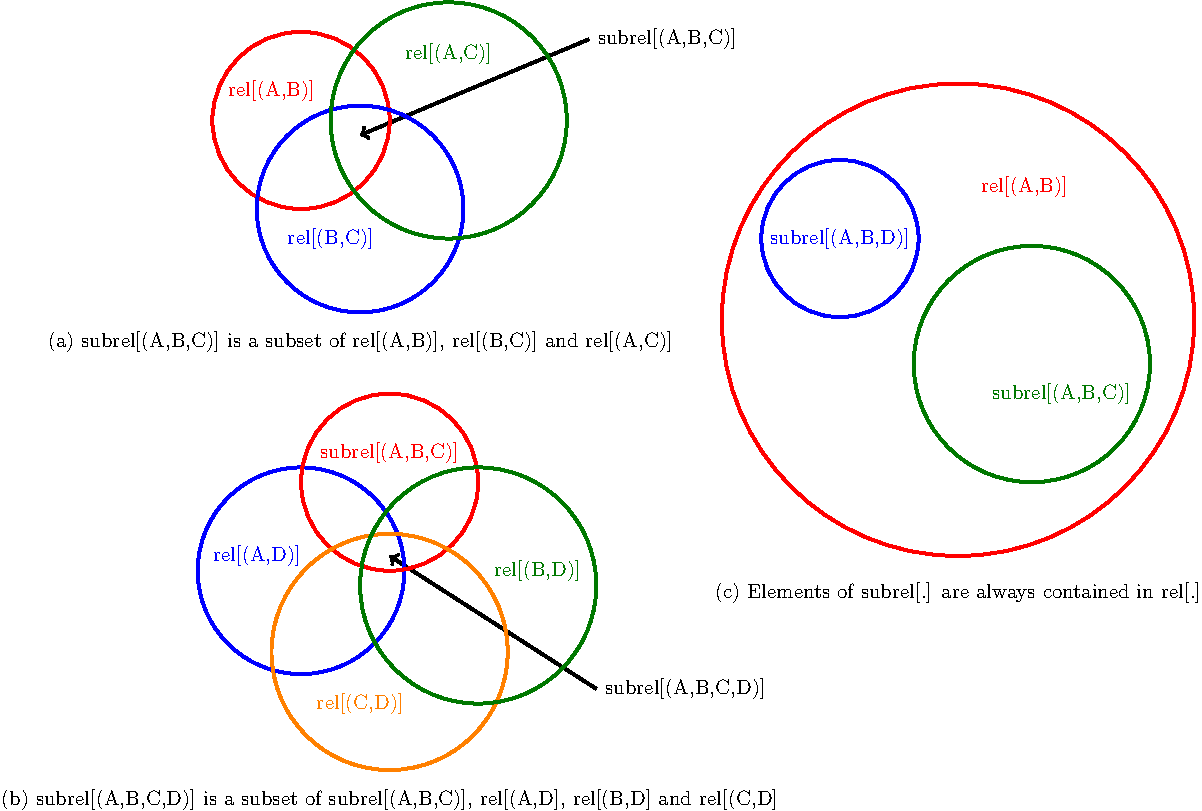
\includegraphics[width=0.5\paperwidth]{E:/Documents/TUM/THESIS/thesisCOD_Ha/figures/rel_example}
\end{figure}

\bibliographystyle{IEEEtran}
\bibliography{../refs/final_ref_bib}

\end{document}
